%======================================================================
\chapter{Hybrid Remote Rendering}
\label{chap:hrr}
%======================================================================

% This part is the abstract of the paper with a minor change.
In this section, we present a hybrid remote rendering framework for applications on mobile devices. In our remote rendering approach, we adopt a client-server model, where the server is responsible for rendering high-fidelity models, encoding the rendering results and sending them to the client, while the client renders low-fidelity models and overlays the high-fidelity frames received from the server on its rendering results. With this configuration, the client is able to keep functioning regardless of network condition and bandwidth. Moreover, to minimize the bandwidth requirements, only key models are rendered in high-fidelity mode. We conduct a user study on factors that may impact the objective and subjective difficulty of an interactive task in a 3D mobile application. The results show that model fidelity has a significant influence on the objective difficulty, while network delay plays an important role in the subjective difficulty. The results of the user study explain how our method is able to benefit the users.

\section{Method}
\label{sec:hrr:m}

\subsection{Client-Server Prototype Design}
\label{sec:hrr:m:cspd}

Our proposed system aims at providing high-quality rendering on less powerful mobile devices, while minimizing the amount of data transferred via the network. We would also like to enable multi-client cooperation to enhance the user experience in training scenarios.

Our system is inspired by Levoy~\cite{levoy1995}, Lamberti and Sanna~\cite{lamberti2007} and Lu et al.~\cite{lu2011} and uses a hybrid approach incorporating both local and remote rendering.
Hence, the low-fidelity key models are stored on the client-side and the local rendering capacity is leveraged to produce lower quality rendering results.
Conversely, the high-fidelity renderings of key models are sent from the server to the client and overlaid upon the locally rendered frames.
Accordingly, the data transferred via the network is minimized due to the small amount of pixels that are sent via the network compared to a CMR solution. 

There are three challenges in realizing multi-client support within the context of the above described system.
First, it is required that the server must not be blocked by any of the clients.
Second, each client has its own view that may be different from all the other clients, this can result in a performance issue as a scene needs to be rendered multiple times in a single animation loop.
Third, because only key models are rendered and sent by the server, occlusion becomes a problem since the environment models that are closer to the viewpoint may not be rendered on the server but just locally.

We address the first problem by mandating that the server interacts with each client independently. More specifically, we enable the server to receive commands from and send to every client separately, so that if a client becomes unresponsive, the server is not blocked.
The second issue is alleviated by implementing a "render-on-demand" function on the server, which means that the server renders the scene for a client only when the client requires a new frame.
We address the third challenge through a two-pass rendering process. In the first pass, the entire scene is rendered in low fidelity on the server. Then the colour buffer is cleared before the second pass where only the key models are rendered in high fidelity. In this way, the second pass is rendered with the depth information obtained from the first pass.

\begin{figure}[!htbp]
	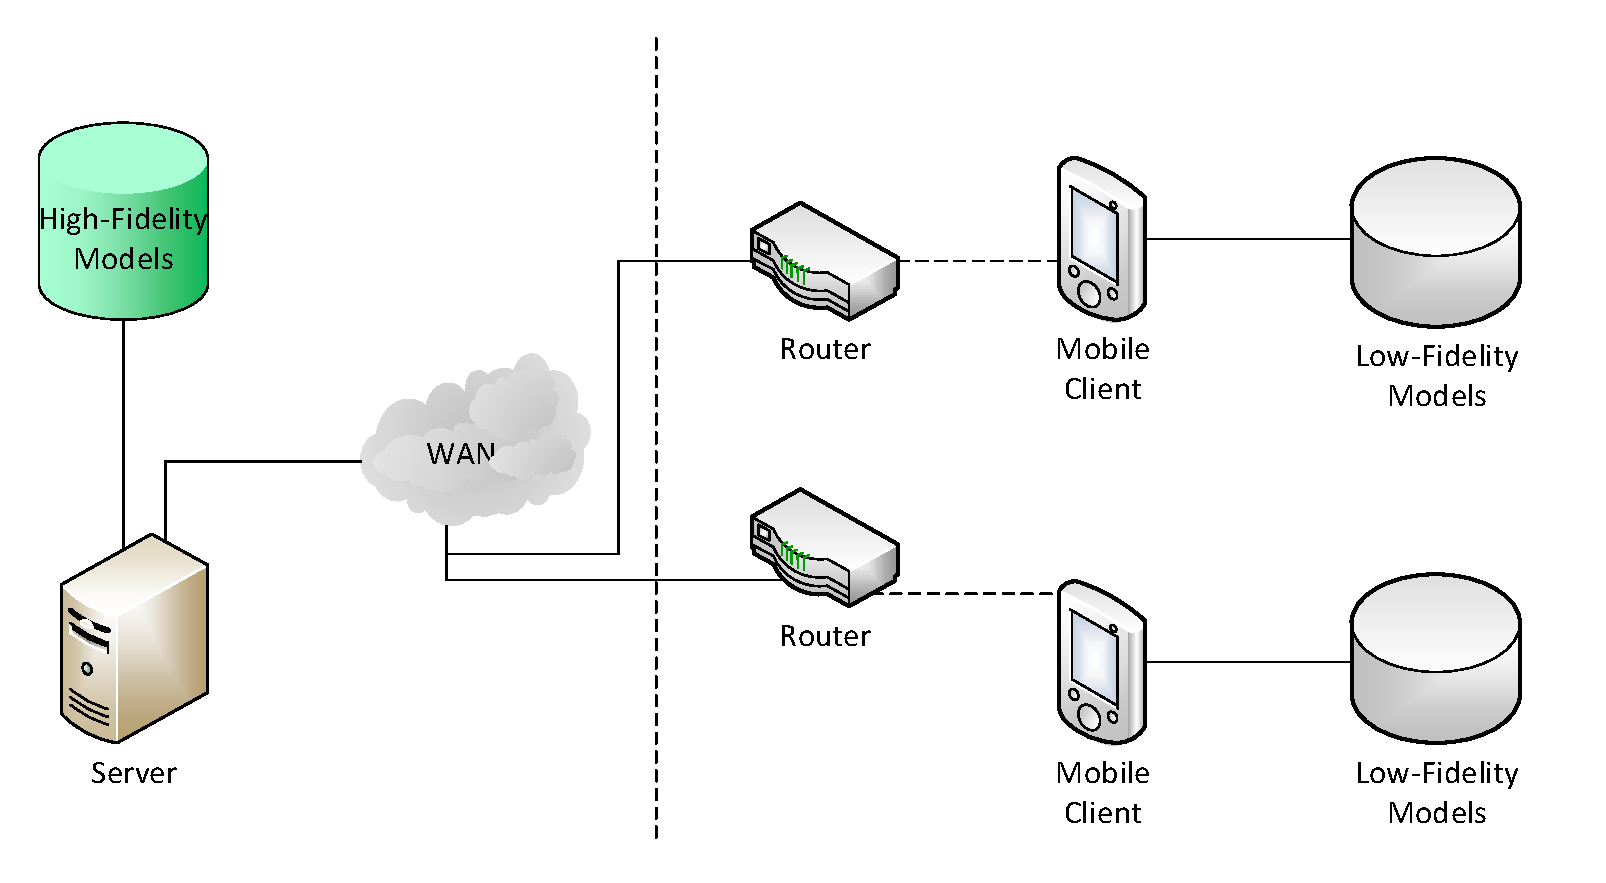
\includegraphics[width=\textwidth]{figures/architecture.pdf}
	\caption{System architecture}
	\label{fig:architecture}
\end{figure}

\begin{figure}[!htbp]
	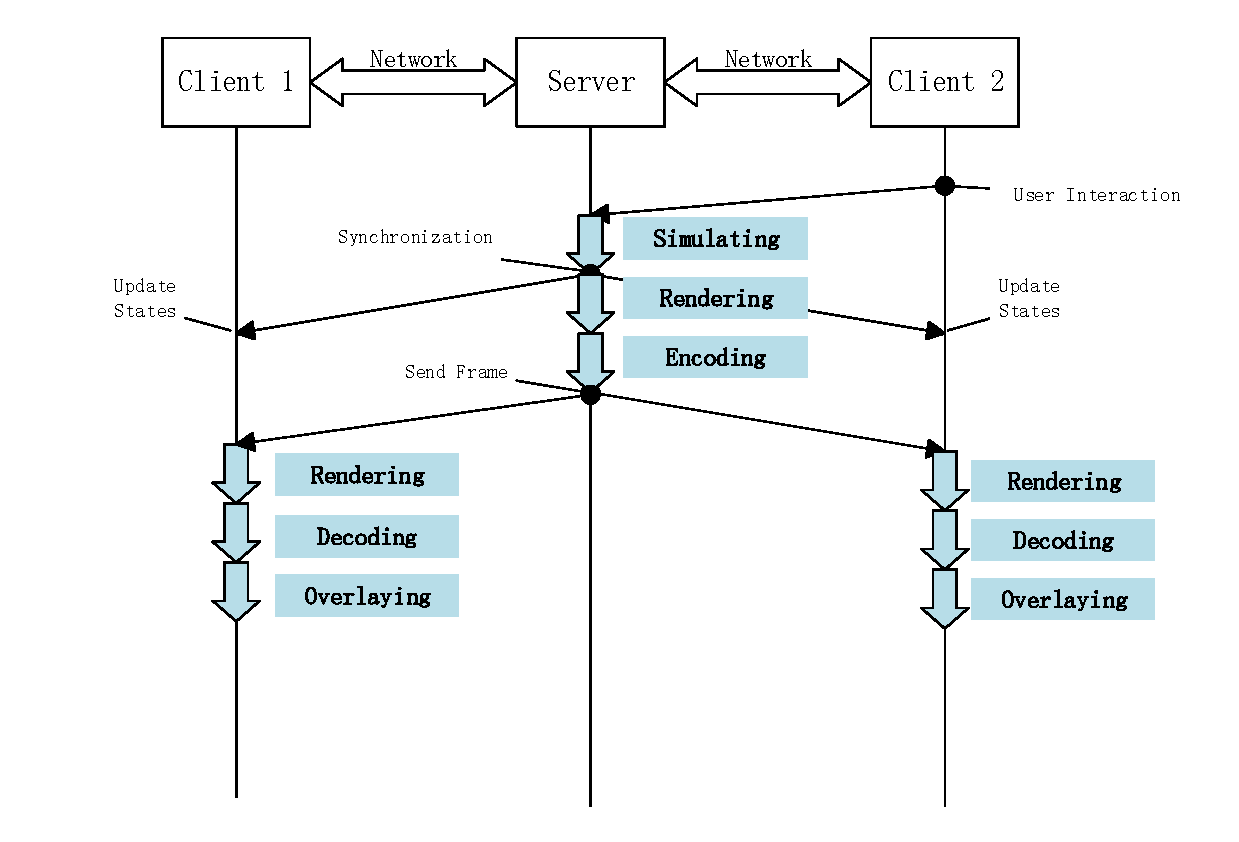
\includegraphics[width=\textwidth]{figures/sequence_workflow.pdf}
	\caption{Workflow of communication between the server and the clients}
	\label{fig:swf}
\end{figure}

As depicted in Fig.~\ref{fig:architecture}, in this system, all clients are connected to the rendering server and send interaction commands to the server.
On the server side, the application status changes according to the commands received from all clients. The application status changes are synchronized with all clients. In this way, the clients are able to cooperate with each other. In other words, when a client changes the status of the application, all clients will see the change after synchronization.
To minimize the amount of transferred data, the client decides which models need to be rendered in high-fidelity and the server only sends the pixels depicting those key models. The other models are still rendered locally.

Fig.~\ref{fig:swf} illustrates the sequence of messages communicated between the server and the client processes. It shows the tasks that are performed by the server and clients to process one frame. If the commands sent from any client influence the simulation states of the server, the latter synchronizes the state changes among all clients to ensure that all of them maintain a consistent state. Moreover, the server renders and encodes the frames for all the clients. Upon receiving the high-fidelity frame, the client decodes and overlays it on the locally rendered frame.

\subsection{Process Behavior}

The proposed system consists of one server and multiple clients.
Fig.~\ref{fig:s-wf} shows the behavior of the server process.
In each loop, the server updates the simulation status of the scene and receives commands from all clients.
Next, the server sends the received commands to all clients to ensure synchronization between them.
On the server side, each client has its own view that is independent from those of the other clients.
The server only renders a new frame upon request from the client.

Fig.~\ref{fig:c-wf} shows the behavior of the client processes. In each loop, the client receives commands from the server and adjusts the simulation status accordingly. Then, it sends its user interaction commands to the server. In each iteration, the client will receive the high-fidelity frame from the server that it has requested in the previous iteration. The client has simplified models stored locally, it renders the scene in every iteration. The high-fidelity frames acquired from the server are overlaid upon the locally rendered frames. Once done, it sends the frame request to the server. In this way, the server does not need to render frames for all clients in every loop, instead it renders a frame when it is needed.

\begin{figure}[!htbp]
	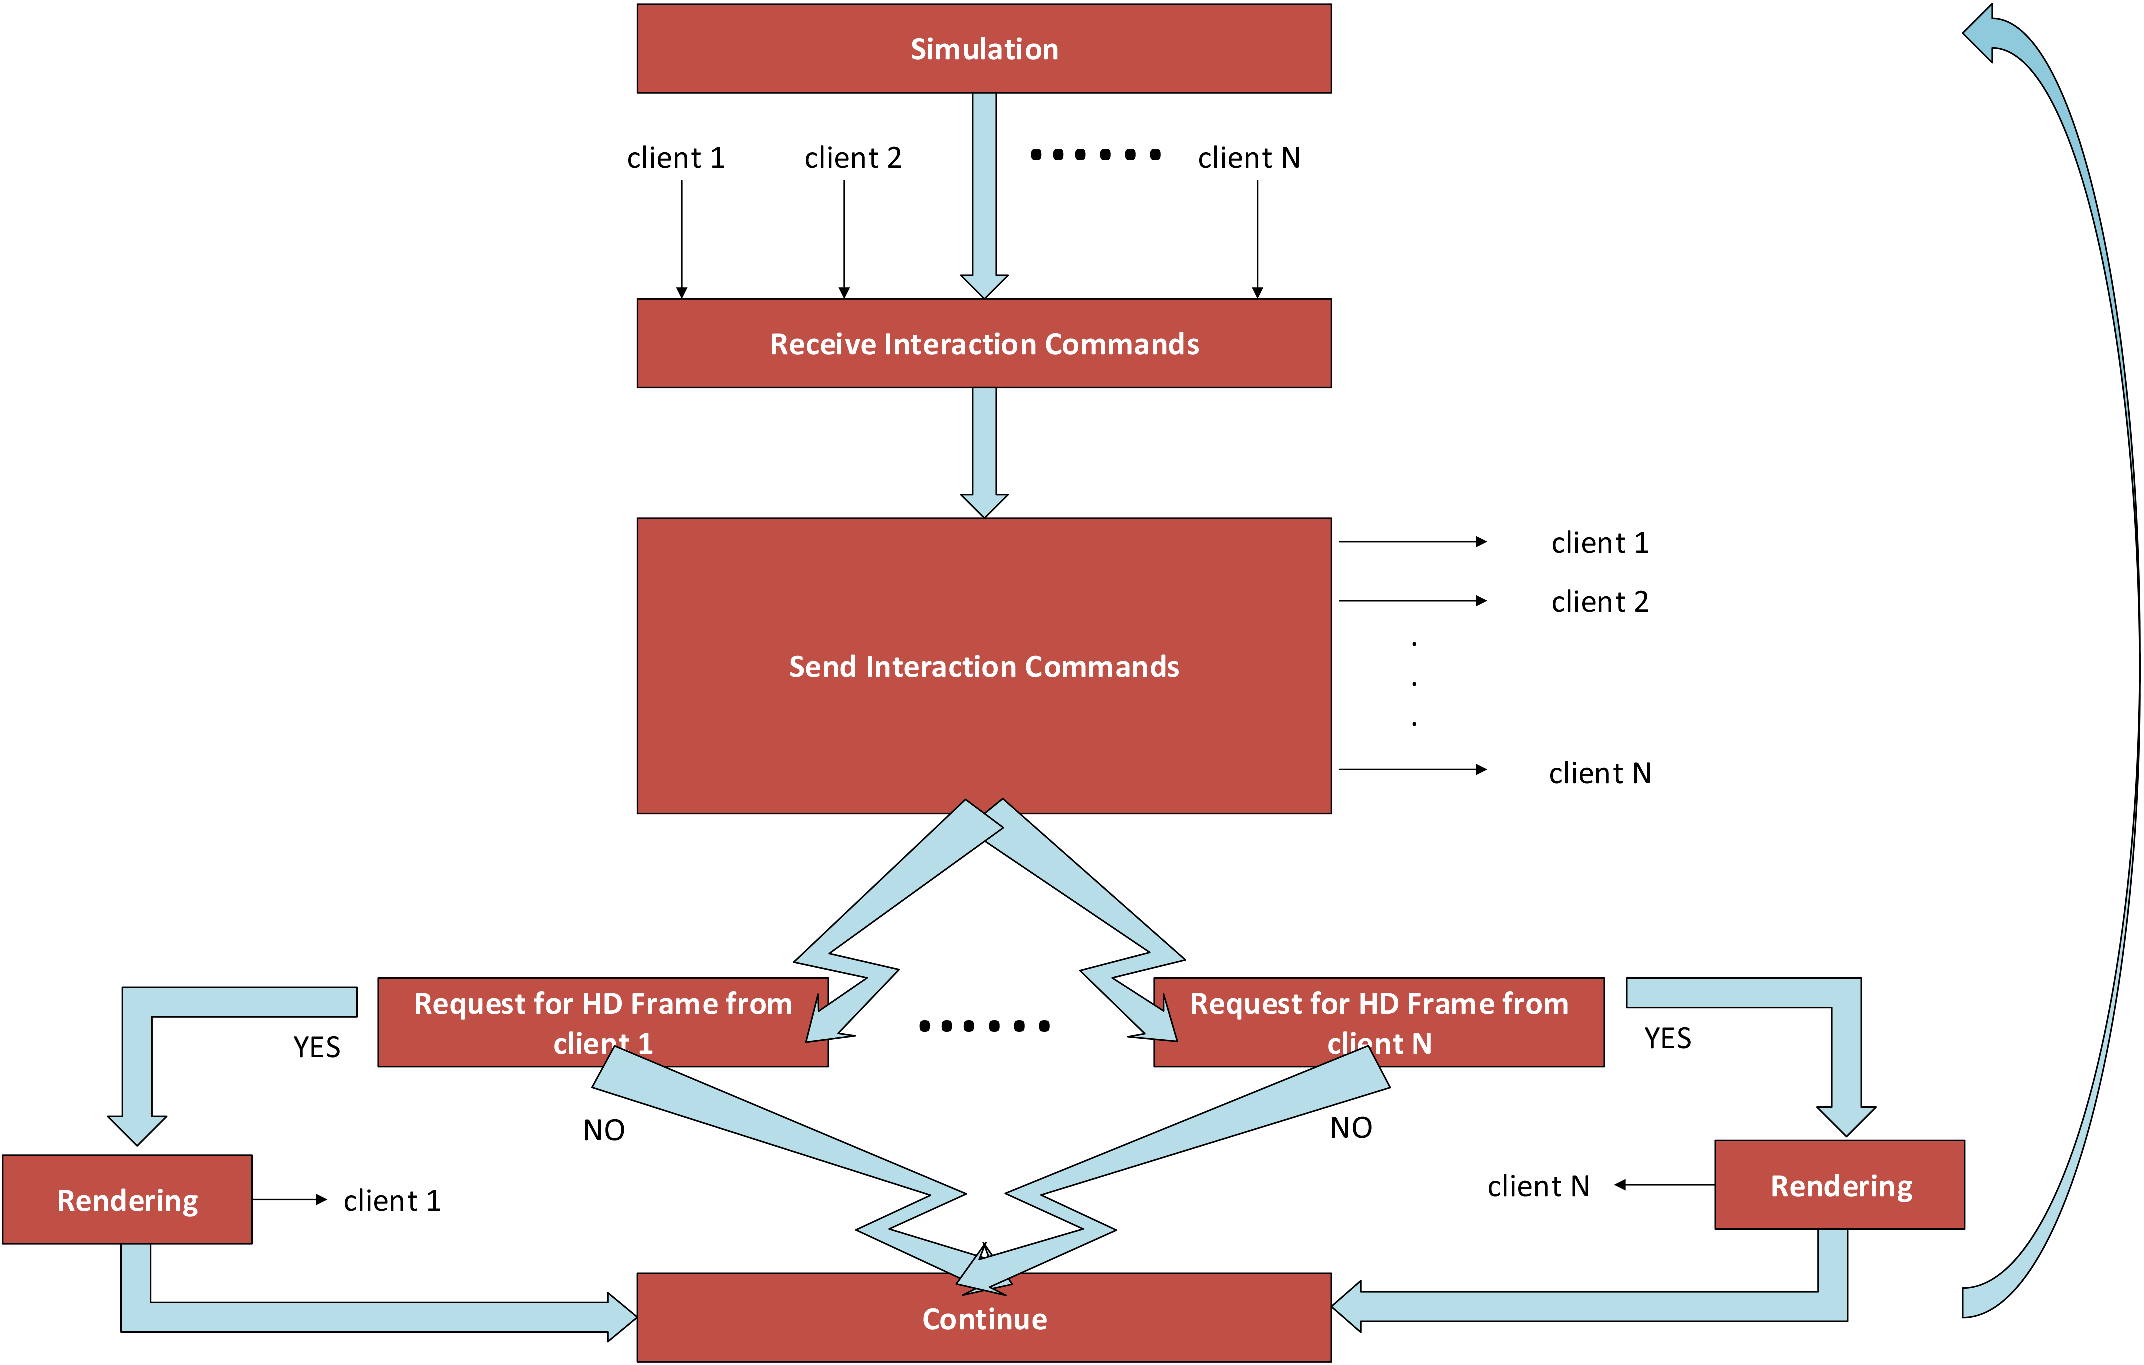
\includegraphics[width=\textwidth]{figures/workflow_server-eps-converted-to.pdf}
	\caption{Server-side Workflow}
	\label{fig:s-wf}
\end{figure}

\begin{figure}[!htbp]
	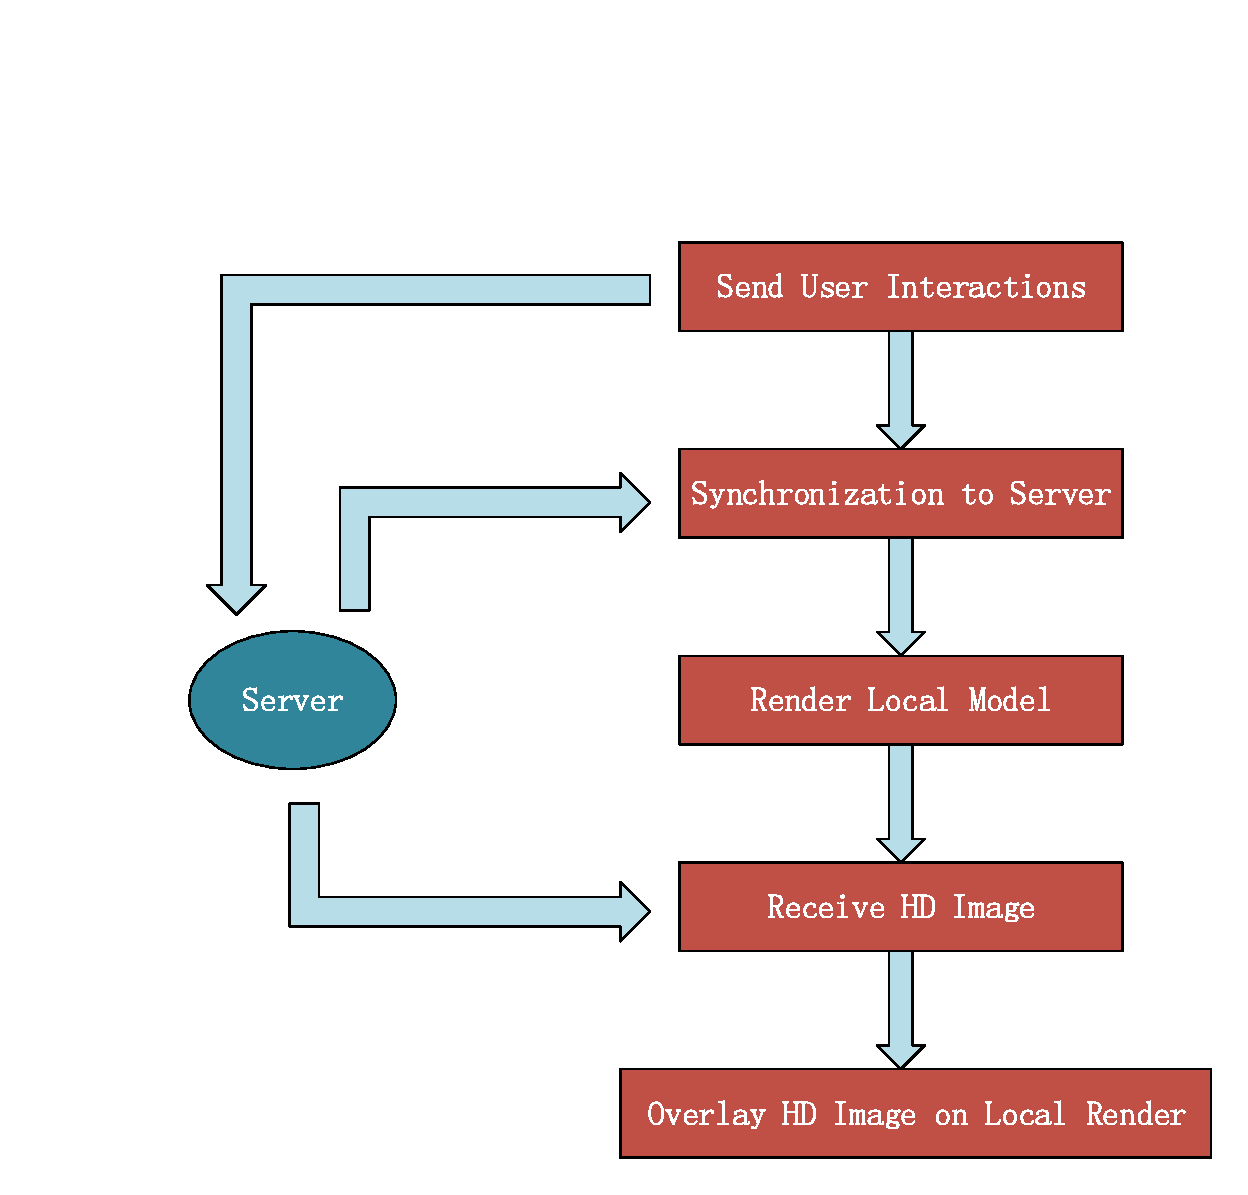
\includegraphics[width=\textwidth]{figures/workflow_client.pdf}
	\caption{Client-side Workflow}
	\label{fig:c-wf}
\end{figure}

\subsection{Two-pass Rendering}

As mentioned in Section~\ref{sec:hrr:m:cspd}, we use a two-pass rendering process on the server side.
The frames sent to the client depict only high-fidelity key models.
But this is not enough for valid view of the 3D scene since other scene content may occlude parts of the key models.
We propose a two-pass rendering process to address this issue.

\begin{figure}[!htbp]
	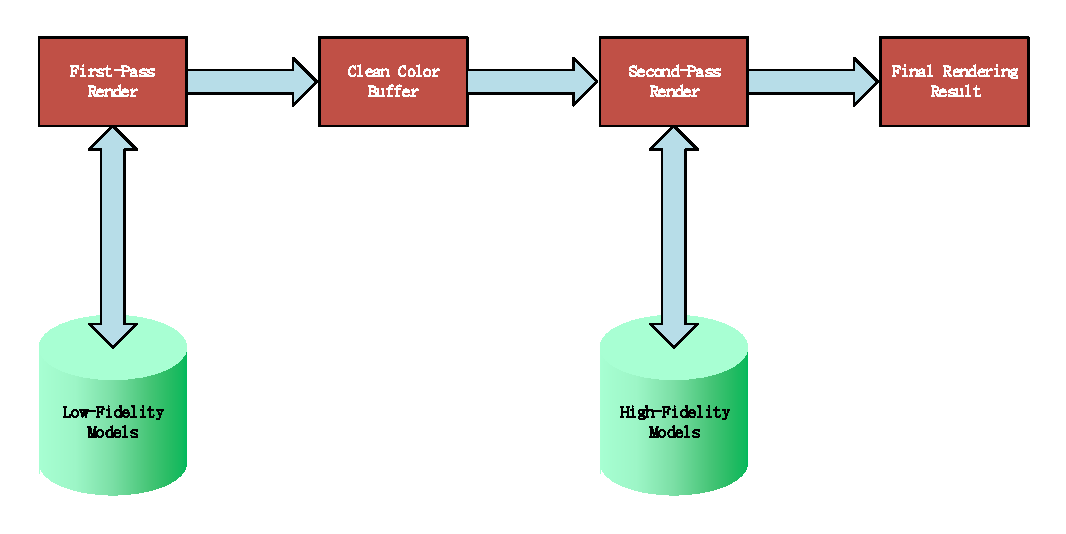
\includegraphics[width=\textwidth]{figures/two-pass-rendering.pdf}
	\caption{Two-pass rendering}
	\label{fig:tp-rendering}
\end{figure}

As shown in Fig.~\ref{fig:tp-rendering}, in the first pass, all models are rendered in low-fidelity except for the key models. Then the color buffer is cleared and only the depth buffer is preserved. In the second pass, only the high-fidelity key models are rendered, while considering the depth information obtained from the first pass rendering, therefore the occlusions are preserved in the final rendered scene.

\subsection{Process Behavior}

The proposed system consists of one server and multiple clients.
Fig.~\ref{fig:s-wf} shows the behavior of the server process.
In each loop, the server updates the simulation status of the scene and receives commands from all clients.
Next, the server sends the received commands to all clients to ensure synchronization between them.
On the server side, each client has its own view that is independent from those of the other clients.
The server only renders a new frame upon request from the client.

Fig.~\ref{fig:c-wf} shows the behavior of the client processes. In each loop, the client receives commands from the server and adjusts the simulation status accordingly. Then, it sends its user interaction commands to the server. In each iteration, the client will receive the high-fidelity frame from the server that it has requested in the previous iteration. The client has simplified models stored locally, it renders the scene in every iteration. The high-fidelity frames acquired from the server are overlaid upon the locally rendered frames. Once done, it sends the frame request to the server. In this way, the server does not need to render frames for all clients in every loop, instead it renders a frame when it is needed.

\begin{figure}[!htbp]
	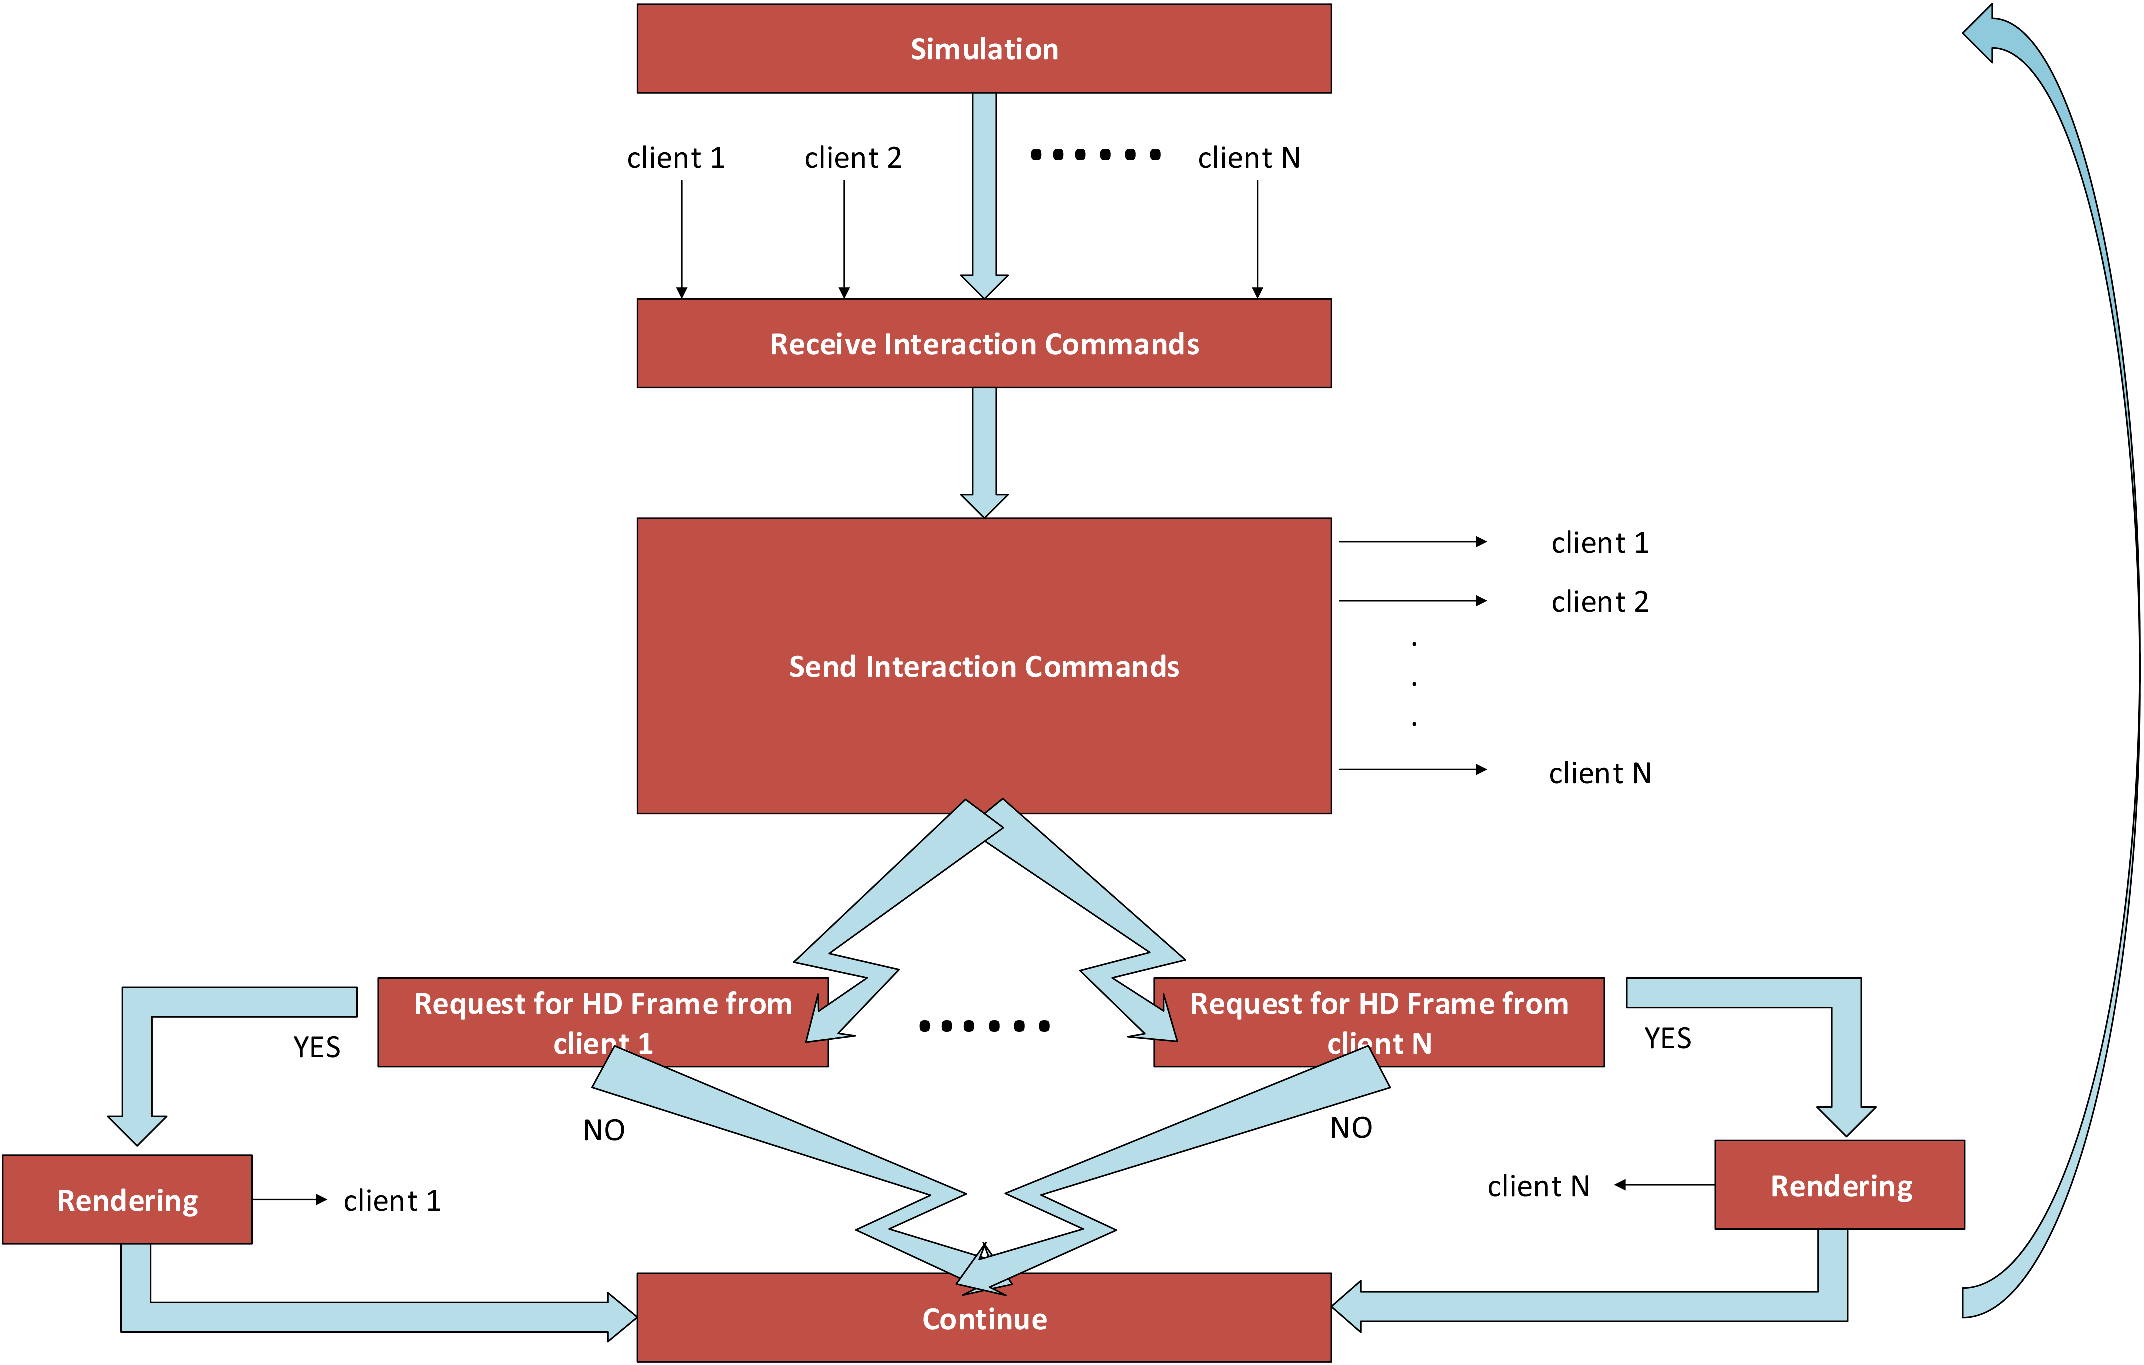
\includegraphics[width=\textwidth]{figures/workflow_server-eps-converted-to.pdf}
	\caption{Server-side Workflow}
	\label{fig:s-wf}
\end{figure}

\begin{figure}[!htbp]
	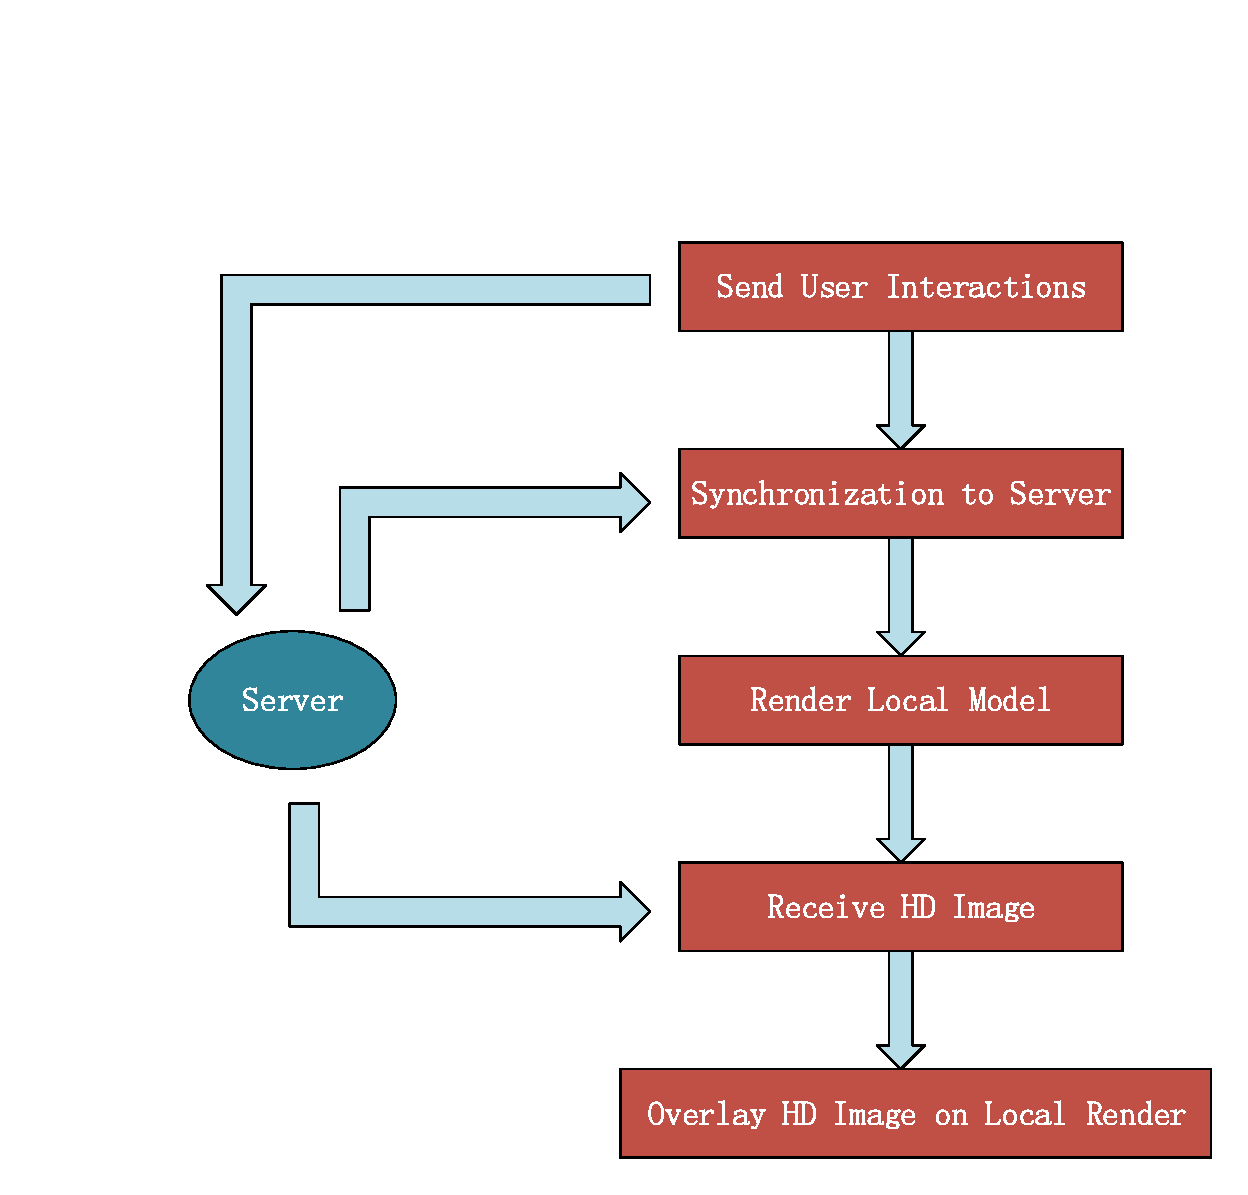
\includegraphics[width=\textwidth]{figures/workflow_client.pdf}
	\caption{Client-side Workflow}
	\label{fig:c-wf}
\end{figure}

\subsection{Two-pass Rendering}

As mentioned in Section~\ref{sec:hrr:m:cspd}, we use a two-pass rendering process on the server side.
The frames sent to the client depict only high-fidelity key models.
But this is not enough for valid view of the 3D scene since other scene content may occlude parts of the key models.
We propose a two-pass rendering process to address this issue.

\begin{figure}[!htbp]
	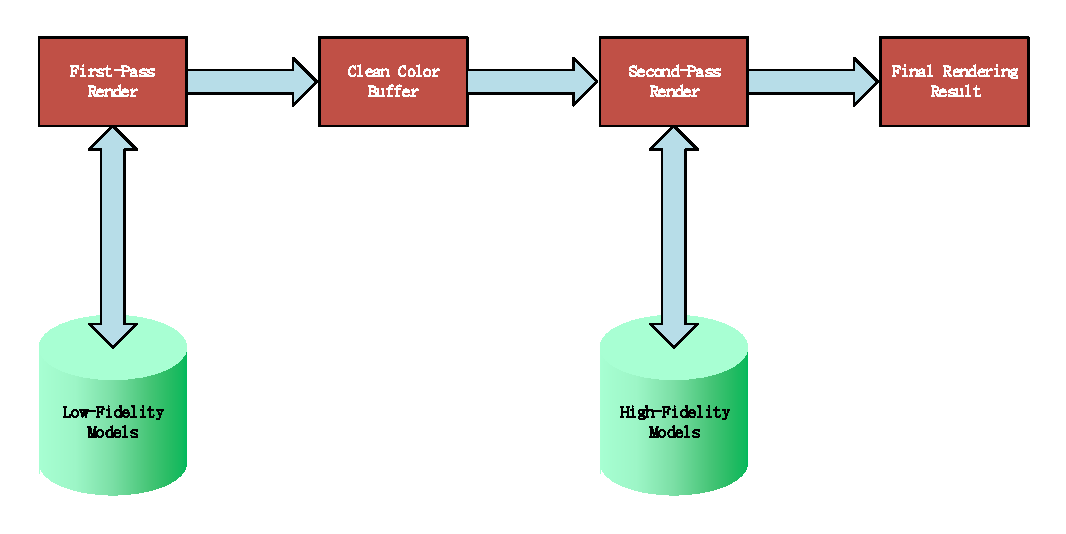
\includegraphics[width=\textwidth]{figures/two-pass-rendering.pdf}
	\caption{Two-pass rendering}
	\label{fig:tp-rendering}
\end{figure}

As shown in Fig.~\ref{fig:tp-rendering}, in the first pass, all models are rendered in low-fidelity except for the key models. Then the color buffer is cleared and only the depth buffer is preserved. In the second pass, only the high-fidelity key models are rendered, while considering the depth information obtained from the first pass rendering, therefore the occlusions are preserved in the final rendered scene.

\section{User Study}
\label{sec:us}

In Section~\ref{sec:hrr:m}, we propose a hybrid remote rendering framework that offloads a part of the rendering task to the remote server. More specifically, only key models are rendered remotely to minimize network bandwidth requirement and network delay.

To overcome the limitations of mobile devices in rendering high-fidelity models, designers often use one of the two approaches:
\begin{enumerate}
\item
Local-only rendering: Reduce the fidelity of the models and render them locally on mobile devices.
\item
Server-only rendering: Render the scene remotely on a server and transfer to the mobile phone client as a video stream.
\end{enumerate}

However, both approaches risk reducing the user's Quality of Experience (QoE). For the local-only rendering approach, the user is interacting with models that are not rendered at their optimal quality. Fine details in the model might be missing, which reduces the aesthetics of the scene. Also, for some applications, these details might carry important information. For instance, it is important for users in many gaming applications to quickly distinguish between similar objects in a scene. Objects rendered as low-fidelity models might not be immediately discernible. For the server-only approach, QoE might be affected by a long delay between the user's actions and application's response. This would be mostly caused by the network delay between client and server. Furthermore, bandwidth limitations can cause interruptions in the video stream.
The proposed approach strikes a balance between local-only rendering and server-only rendering. It renders only key models remotely at high-fidelity while other models are rendered locally at low-fidelity. 

Previous work has explored how various factors affect the user experience. Hong et al.~\cite{hong2015user-study} conducted a subjective user study to quantify the effect that video bitrate and frame rate have on QoE in cloud gaming.
Slivar et al.~\cite{slivar2015qoe} use Steam In-home streaming platform\footnote{http://store.steampowered.com/streaming/} as a case to study how the frame rate and bitrate influence the QoE. They model the QoE as a combination of two aspects: perceived graphics quality and perceived game fluidity.
In the work by Suznjevic et al.~\cite{suznjevic2016}, five factors (i.e. latency, jitter, packet loss, frame rate and frame resolution) are studied in terms of their effects on the QoE of NVIDIA GeForce Now platform.
Hemmati et al.~\cite{hemmati2013bitrate} developed an algorithm that minimizes bitrate by not rendering unimportant models. Our method leverages a similar idea by rendering key models in high fidelity and environment models in low fidelity. But the difference is that our method renders the environment models locally instead of not rendering them at all.

Our method targets not only gaming, but also other types of applications, such as training applications and virtual tours. The expectations of users in terms of graphics quality and application fluidity may depend on the different types of applications. For instance, the players of a game may focus on the quality of special effects, while the users of a surgery application may focus on how clearly anatomical features can be distinguished. Thus, we do not measure QoE but how difficult it is to accomplish a given task. Thus, we are interested in the effects of the key model fidelity and environment fidelity on the perceived diffculty of task completion. We name this measure the Difficulty of Task (DoT). We measure DoT in two ways: Objective DoT (ODoT) and Subjective DoT (SDoT).
The ODoT is a measure of how well the users can accomplish a task. It might be measured by a score or a level calculated by the application.
The SDoT is a measure of the users' opinion on the task difficulty and can be answered by a subjective questionnaire.

Our user study was approved by the Research Ethics Board at the University of Ottawa (File Number: H12-16-05).
The main user study is informed by a pre-trial study discussed next.

\subsection{Pre-Trial Study}
\label{sec:hrr:us:pts}

A major goal of the main study is to analyze the effect of 3D model fidelity on the DoT. However, in the proposed framework, there are two types of models, high-fidelity models and low-fidelity models. Those models will be used in the main study (see Section~\ref{sec:hrr:us:ms}). We have prepared 15 high-fidelity models and simplified them to obtain low-fidelity models using QSlim~\cite{garland1997}.

\subsubsection{Objective}

The objective of the pre-trial study is to decide the number of polygons for the low-fidelity models. If it is too low, the participants will not be able to recognize the object that the model represents. In the pre-trial study, we want to find out at which point the object represented by the model becomes discernible to the majority or all subjects.

\subsubsection{Participants}

We recruited 5 participants, 4 males and 1 female. None of the subjects were visually impaired.

\subsubsection{Independent Variables and Dependent Measures}
\label{sec:hrr:us:pts:ivdm}

The experiment was conducted with one independent variable: number of polygons of the surface mesh in the 3D model.
The independent variable has 50 levels. For the first level, the model is composed of 20 polygons. For each of the 49 subsequent levels, the number of polygons is increased by $10\%$. We measure the number of polygons necessary for a subject to recognize the object for each 3D model.

\subsubsection{Procedure}

The experiment was conducted using a program that shows 15 models at different levels of fidelity.  We create 50 levels of fidelity for each model by starting with 20 polygons and increasing its polygon count by $10\%$ for every level using QSlim~\cite{garland1997}. Our program shows the subjects a model on the screen and asks them to select the object it represents from a side menu by choosing among dog, cat, horse, or unknown. Subjects were instructed to choose the unknown option if they were unsure. We start with a model with very low polygon count (20 polygons). Every time the subject selects an answer, we increase the polygon count to the next level adding more details to the model. The order through which the models are shown to the subjects is randomized to avoid biasing the results. 

\subsubsection{Results}

\begin{table}[!htbp]
\caption{Data collected from the pre-trial study, which represents the number of polygons above which a participant ceases to make mistakes are shown. However, in one case, one of the participants does not recognize the model even at full resolution (marked by a dash). The numbers in bold are those selected as the final number of polygons of the low-fidelity models for the main study.}
\label{tab:pts}
\begin{tabular}{llllll}
\hline\noalign{\smallskip}
& Participant \#1 & Participant \#2 & Participant \#3 & Participant \#4 & Participant \#5 \\
\noalign{\smallskip}\hline\noalign{\smallskip}
Model \#1 & 148 & 22 & 57 & 51 & \textbf{111} \\
Model \#2 & 162 & 57 & \textbf{422} & 22 & 422 \\
Model \#3 & 122 & 383 & 134 & 22 & \textbf{238} \\
Model \#4 & 75 & \textbf{148} & - & 69 & 134 \\
Model \#5 & 162 & 51 & 32 & 22 & \textbf{134} \\
Model \#6 & \textbf{1095} & 179 & 464 & 1940 & 464 \\
Model \#7 & 995 & 1603 & \textbf{1325} & 32 & 422 \\
Model \#8 & 75 & 162 & 148 & 91 & \textbf{148} \\
Model \#9 & 75 & 83 & 216 & 122 & \textbf{196} \\
Model \#10 & 464 & 262 & 748 & 216 & \textbf{562} \\
Model \#11 & 422 & 1204 & \textbf{422} & 288 & 383 \\
Model \#12 & 47 & 101 & \textbf{134} & 22 & 134 \\
Model \#13 & 22 & 47 & 510 & 29 & \textbf{238} \\
Model \#14 & 238 & 22 & 348 & \textbf{317} & 162 \\
Model \#15 & 69 & 83 & \textbf{75} & 75 & 51 \\
\noalign{\smallskip}\hline
\end{tabular}
\end{table}

Table~\ref{tab:pts} contains the data collected from the pre-trial study. The number of polygons above which a participant ceases to make mistakes (i.e. the participant choses the correct answer consistently at all further levels of fidelity). The data are used to decide the number of polygons for the low-fidelity models in the main study. To eliminate the outliers, we select the second highest number among all participants for each model.

\subsection{Main Study}
\label{sec:hrr:us:ms}

Our main user study is designed to address the following research questions:
\begin{enumerate}
\item
What is the effect of key model fidelity on the DoT?
\item
What is the effect of environment model fidelity on the Dot?
\item
What is the effect of network delay on the DoT?
\item
What is the effect of network jitter on the DoT
\end{enumerate}

We ask the subjects to interact with a 3D mobile application that prompts the user to respond rapidly to visual stimuli. This is a stand-in for a variety of applications that require the user to react swiftly to changing aspects in a 3D environment. Examples of such applications are games, flight simulators, military training systems, etc... We compare our results to conventional server-only and local-only rendering approaches. In our user study, we do not consider any network-aware adaption strategies of the video stream performed by the remote server.

The test application we use in our experiment depicts a 3D environment representing a virtual room. Guided by a compass, the user must navigate (pan and tilt) the environment to reach a destination at which an object will appear and disappear within a short period of time.
A menu prompting the user to specify the type of that object is brought up after an object appears, as shown in Fig.~\ref{fig:us}.
This test application is designed as a simplification of a large variety of 3D applications. It consists of two sub-tasks: navigation and recognition.
For instance, in a 3D shooting game, the players move around in the environment and look for his/her targets. After finding a target, the players need further recognize the targets to decide whether it is an enemy or a friend.
Another example is surgery training applications~\cite{cecil2013}, in which the users need to navigate to change the view point and recognize different components of the body before performing an action.

\subsubsection{Hypothesis}

We devise eight null hypotheses to test in the experiment, see Table~\ref{tab:hypo}. The null hypotheses are defined for each measurement factor. In those null hypotheses, we assume all four factors do not have any effect on the ODoT nor the SDoT. Rejecting a null hypothesis indicates that there is no evidence proving that the corresponding factor has no effect on that dependent measure.

\begin{table}[!htbp]
\caption{Hypotheses.}
\label{tab:hypo}
\begin{tabular}{ll}
\noalign{\smallskip}\hline\noalign{\smallskip}
H\textsubscript{01} & Different model fidelities do not affect the ODoT \\
H\textsubscript{02} & Different environment fidelities do not affect the ODoT \\
H\textsubscript{03} & Different network delays do not affect the ODoT \\
H\textsubscript{04} & Existence of jitter does not affect the ODoT \\
H\textsubscript{05} & Different model fidelities do not affect the SDoT \\
H\textsubscript{06} & Different environment fidelities do not affect the SDoT \\
H\textsubscript{07} & Different network delays do not affect the SDoT \\
H\textsubscript{08} & Existence of jitter does not affect the SDoT \\
\noalign{\smallskip}\hline
\end{tabular}
\end{table}

\subsubsection{Participants}

15 volunteers participated in the main study, 12 males and 3 females. None of the subjects were visually impaired.

\subsubsection{Independent Variables and Dependent Measures}
\label{sec:hrr:us:ms:ivdm}

The experiment was conducted with four independent variables: key model fidelity, environment model fidelity, delay and jitter.
Key model fidelity and environment model fidelity have two levels: high and low, as described in Section~\ref{sec:hrr:us:pts}.
The variable delay is set to introduce network delay. In the variable network delay, we summarize the effects of network transmission, remote rendering and encoding. In this experiment, the variable delay was simulated locally. Similar to the work by Zhu et al.~\cite{zhu1998jitter}, we use the normal distribution of (\ref{equ:jitter}) for jitter in settings with non-zero delay.

\begin{equation}
\label{equ:jitter}
p(j|\mu,\sigma^{2})=\frac{1}{\sqrt{2\pi\sigma^{2}}}^{-\frac{(j-\mu)^{2}}{2\sigma^{2}}}
\end{equation}
where j is the value of jitter, $\mu=77\mathrm{ms}$ and $\sigma^{2}=1$.

Combining the four variables results in 20 configurations. Table~\ref{tab:pus} details the test application configurations. The order of the 20 configurations is randomized across subjects to avoid biasing the results.

\begin{table}[!htbp]
\caption{Test application configurations.}
\label{tab:pus}
\begin{tabular}{lllll}
\hline\noalign{\smallskip}
Configuration & Key Model Fidelity & Environment Model Fidelity & Delay & Jitter \\
\noalign{\smallskip}\hline\noalign{\smallskip}
1 & low & low & $0\mathrm{ms}$ & not applicable \\
2 & low & high & $0\mathrm{ms}$ & not applicable \\
3 & high & low & $0\mathrm{ms}$ & not applicable \\
4 & high & high & $0\mathrm{ms}$ & not applicable \\
5 & low & low & $80\mathrm{ms}$ & not applied \\
6 & low & high & $80\mathrm{ms}$ & not applied \\
7 & high & low & $80\mathrm{ms}$ & not applied \\
8 & high & high & $80\mathrm{ms}$ & not applied \\
9 & low & low & $80\mathrm{ms}$ & applied \\
10 & low & high & $80\mathrm{ms}$ & applied \\
11 & high & low & $80\mathrm{ms}$ & applied \\
12 & high & high & $80\mathrm{ms}$ & applied \\
13 & low & low & $120\mathrm{ms}$ & not applied \\
14 & low & high & $120\mathrm{ms}$ & not applied \\
15 & high & low & $120\mathrm{ms}$ & not applied \\
16 & high & high & $120\mathrm{ms}$ & not applied \\
17 & low & low & $120\mathrm{ms}$ & applied \\
18 & low & high & $120\mathrm{ms}$ & applied \\
19 & high & low & $120\mathrm{ms}$ & applied \\
20 & high & high & $120\mathrm{ms}$ & applied \\
\noalign{\smallskip}\hline
\end{tabular}
\end{table}

In this experiment, we collect two types of data: ODoT and SDoT.
The ODoT is measured by the number of objects that participants incorrectly recognize.
The SDoT is measured using a questionnaire directly integrated within the test application. The questionnaire contains one question: "Please score how difficult it was to complete the task". A 5 point Likert Scale is used to collect the answers. A score between 1 to 5 is associated with each question, where 1 represents the option "Very Easy" and 5 represents the option "Very Difficult".

\subsubsection{Procedure}

We run the test application 20 times for each subject. We vary the key model fidelity, environment model fidelity, delay and jitter across these runs. Table~\ref{tab:pus} details the test application configurations for the 20 runs. The order of the 20 configurations is randomized across subjects to avoid biasing the results.
For each configuration, ten 3D objects appear. So the maximum score of the ODoT for each configuration is 10 and the minimum score is 0.
As mentioned in Section~\ref{sec:hrr:us:ms:ivdm}, we also collect SDoT during the experiment. After each run of the test application, the participant was asked to fill the SDoT questionnaire.

As shown in Table~\ref{tab:pus}, we prepare four types of scenes: a scene with only low-fidelity key models and low-fidelity environment models, a scene with low-fidelity key models and high-fidelity environment models, a scene with high-fidelity key models and low-fidelity environment models and a scene with high-fidelity key models and high-fidelity environment models. We simulate three different network delays: $0\mathrm{ms}$, $80\mathrm{ms}$ and $120\mathrm{ms}$ and we also consider network jitter.

\begin{figure}
	\centering
	\subfigure[Sub-task of navigation]{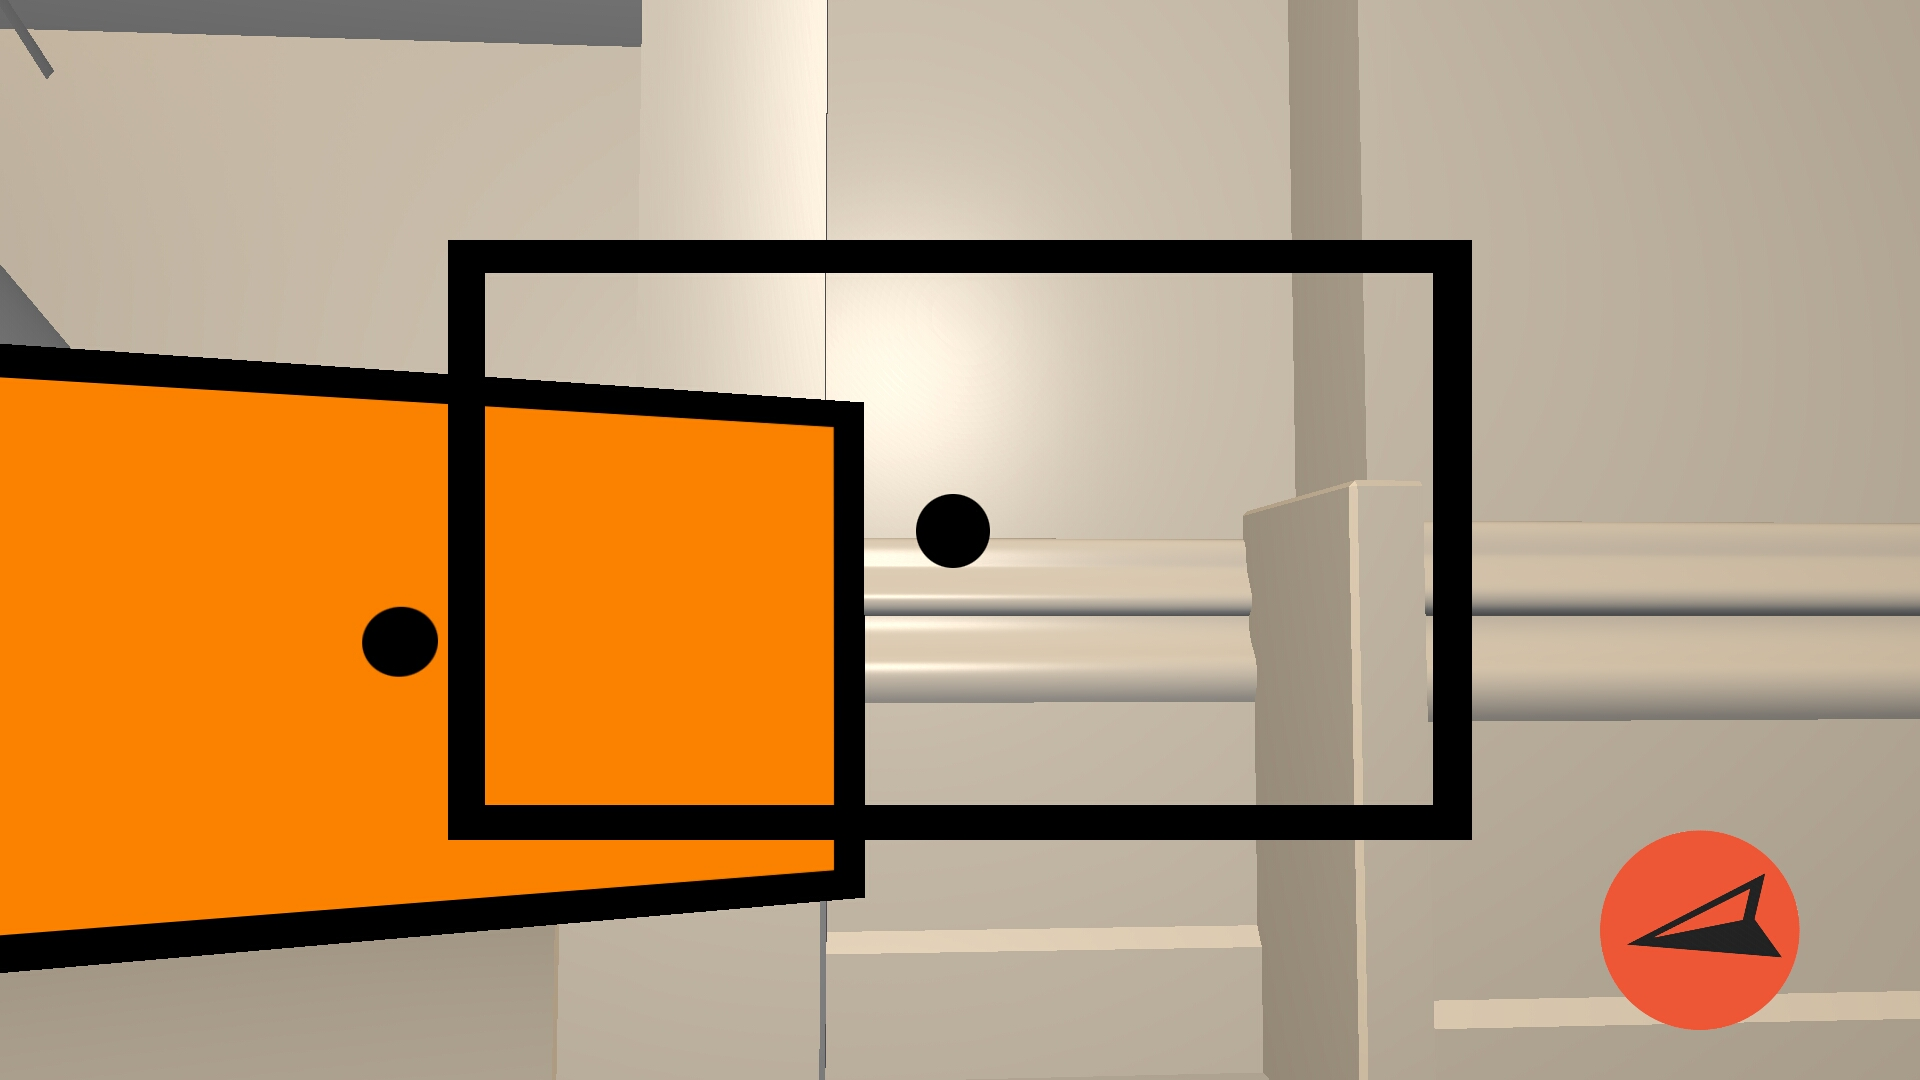
\includegraphics[width=0.49\columnwidth]{figures/user_study_screen_shot1.jpg}}
	\subfigure[Sub-task of recognition]{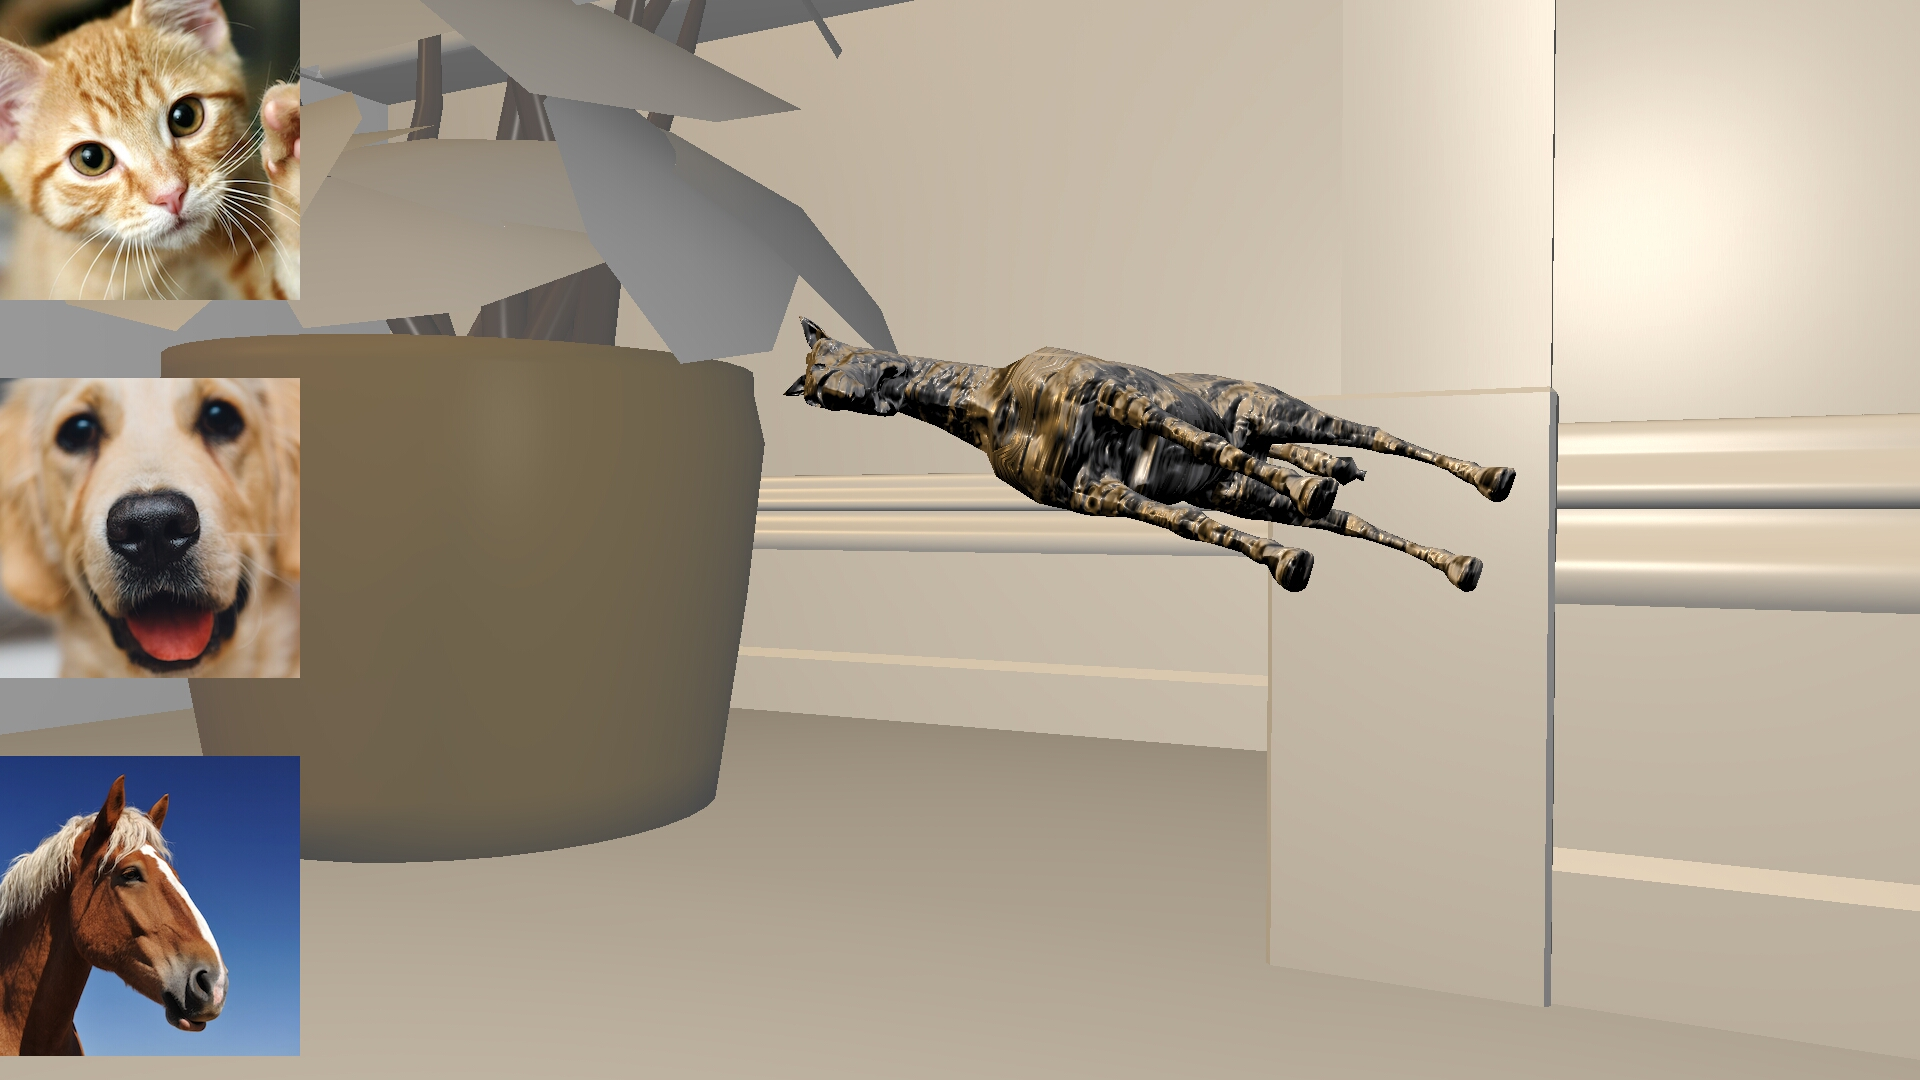
\includegraphics[width=0.49\columnwidth]{figures/user_study_screen_shot2.jpg}}
	\caption{Screenshots of the test application. During one run of the test application, the two sub-tasks are repeated ten times with different animal models. (a) Sub-task of navigation. In the test application, users need to pan and tilt to align the camera viewfinder with the orange plate by following the direction of the compass. If there exist network delay and jitter, users will feel them when panning and tilting. (b) Sub-task of recognition. After aligning the camera viewfinder with the plate, an object appears. The object is not static, but rotating and moving around instead. As similar to the sub-task of navigation, the movement and rotation of the object is also influenced by network delay and jitter.}
	\label{fig:us}
\end{figure}

\subsubsection{Results}
\label{sec:hrr:us:r}

To understand how each factor affects the SDoT and the ODoT, we use analysis of variance (ANOVA) to interpret our experimental data.

We use a four-way ANOVA test to investigate the effect of all four factors. However the factor combination of delay and jitter is not complete, since jitter is not applicable when delay is $0\mathrm{ms}$. So we exclude the delay level $0\mathrm{ms}$ in the four-way ANOVA test.
As shown in Table~\ref{tab:fal}, the four-way ANOVA considers the four factors and their levels, except for $0\mathrm{ms}$ of delay.

We also analyze the effect of the delay factor and its interaction with key model fidelity and environment model fidelity. For this analysis, we resort to a three-way ANOVA for the combination of delay, key model fidelity and environment model fidelity. Table~\ref{tab:fal} shows the factors of the three way ANOVA.

\begin{table}[!htbp]
\caption{Factors and levels of the ANOVA tests.}
\label{tab:fal}
\begin{tabular}{llllllllll}
\hline\noalign{\smallskip}
& \multicolumn{2}{c}{\makecell{Key Model\\Fidelity}} & \multicolumn{2}{c}{\makecell{Environment\\Model\\Fidelity}} & \multicolumn{3}{c}{Delay} & \multicolumn{2}{c}{Jitter} \\
\noalign{\smallskip}\hline\noalign{\smallskip}
& Low & High & Low & High & $0\mathrm{ms}$ & $80\mathrm{ms}$ & $120\mathrm{ms}$ & applied & not applied \\
\noalign{\smallskip}\hline\noalign{\smallskip}
Four-way ANOVA & \cmark & \cmark & \cmark & \cmark & \xmark & \cmark & \cmark & \cmark & \cmark \\
Three-way ANOVA & \cmark & \cmark & \cmark & \cmark & \cmark & \cmark & \cmark & \xmark & \xmark \\
\noalign{\smallskip}\hline
\end{tabular}
\end{table}

Table~\ref{tab:mou} shows the grand mean of the ODoT measure for all factors. The ODoT refers to the number of objects the user did not recognize, hence higher scores represent higher objective difficulty of task. Since we employ two tests of significance (four-way and a three-way ANOVA) we calculate two grand means of the ODoT for each factor level. Four-way ANOVA does not consider the results of configurations 1 to 4 of Table~\ref{tab:pus} (since it does not consider $0\mathrm{ms}$ delay as previously explained). Table~\ref{tab:mou} shows that the ODoT varies with different levels of each factor. However, not all factors have an effect on the ODoT.
We can see that in both, the four-way and the three-way ANOVA, participants are able to reduce the number of incorrectly recognized objects with high-fidelity key models and in low-fidelity environment models.
% and jitter.
The grand means for the factor delay do not agree in the four-way ANOVA and the three-way ANOVA, so we consider the factor delay as not having an effect on ODoT.

Table~\ref{tab:mom} shows the grand means with respect to SDoT. As in Table~\ref{tab:mou}, we show the grand means calculated for the four-way ANOVA and three-way ANOVA tests in Table~\ref{tab:mom}. The means are measured through a 5 point Likert Scale, where larger values indicate higher subjective difficulty of task.

From Table~\ref{tab:mom}, we can see that three factors have effects on the SDoT. The SDoT is reduced for high-fidelity key models and low delay.
% and jitter.
The grand means for the factor environment model fidelity do not agree in the four-way ANOVA and the three-way ANOVA, so we cannot conclude that the factor environment model fidelity has an effect on SDoT.

\begin{table}[!htbp]
\caption{Grand means of the ODoT for each factor.}
\label{tab:mou}
\begin{tabular}{llllllllll}
\hline\noalign{\smallskip}
& \multicolumn{2}{c}{\makecell{Key Model\\Fidelity}} & \multicolumn{2}{c}{\makecell{Environment\\Model\\Fidelity}} & \multicolumn{3}{c}{Delay} & \multicolumn{2}{c}{Jitter} \\
\noalign{\smallskip}\hline\noalign{\smallskip}
& low & high & low & high & $0\mathrm{ms}$ & $80\mathrm{ms}$ & $120\mathrm{ms}$ & applied & not applied \\
\noalign{\smallskip}\hline\noalign{\smallskip}
Four-way ANOVA & 4.6 & 3.5 & 3.9 & 4.2 & - & 4.0 & 4.1 & 3.8 & 4.2 \\
Three-way ANOVA & 4.3 & 3.5 & 3.8 & 4.0 & 4.0 & 3.9 & 3.8 & - & - \\
\noalign{\smallskip}\hline
\end{tabular}
\end{table}

\begin{table}[!htbp]
\caption{Grand means of the SDoT for each factor.}
\label{tab:mom}
\begin{tabular}{llllllllll}
\hline\noalign{\smallskip}
& \multicolumn{2}{c}{\makecell{Key Model\\Fidelity}} & \multicolumn{2}{c}{\makecell{Environment\\Model\\Fidelity}} & \multicolumn{3}{c}{Delay} & \multicolumn{2}{c}{Jitter} \\
\noalign{\smallskip}\hline\noalign{\smallskip}
& low & high & low & high & $0\mathrm{ms}$ & $80\mathrm{ms}$ & $120\mathrm{ms}$ & applied & not applied \\
\noalign{\smallskip}\hline\noalign{\smallskip}
Four-way ANOVA & 2.7 & 2.5 & 2.7 & 2.6 & - & 2.5 & 2.8 & 2.5 & 2.7 \\
Three-way ANOVA & 2.4 & 2.2 & 2.2 & 2.3 & 1.9 & 2.4 & 2.6 & - & - \\
\noalign{\smallskip}\hline
\end{tabular}
\end{table}

However, the conclusions drawn from Table~\ref{tab:mou} and Table~\ref{tab:mom} may not be significantly different in statistics.
% It is probably caused by the small number of samples. 
Hence, we analyze the variance for both metrics, i.e. ODoT and SDoT to determine whether any of the differences between the means are statistically significant, we compare the $p$-values to a significance level to decide whether the $p$-value suggests accept or reject on the null hypothesis. We choose a significance level of 0.05.

Table~\ref{tab:fau} and Table~\ref{tab:tau} demonstrate the results of ANOVA in terms of the ODoT, where Table~\ref{tab:fau} shows the results of the four way ANOVA while Table~\ref{tab:tau} shows the results of the three way ANOVA.

Only the key model fidelity factor exhibits a $p$-value less than 0.05 for both ANOVA tests for the ODoT measure.
To explore the interaction between a factor pair or among multiple factors, we also calculate the $p$-values for those interactions.
These kind of calculations are performed for every combination of factors, including combination of two factors, combination of three factors, and combination of four factors if plausible.
From Table~\ref{tab:fau} and Table~\ref{tab:tau}, we can see that there is no combination whose $p$-value is smaller than 0.05.
This indicates that these factors are independent from each other in terms of the ODoT.

\begin{table}[!htbp]
\caption{Four-way ANOVA of the ODoT.}
\label{tab:fau}
\begin{tabular}{lll}
\hline\noalign{\smallskip}
Source & F-statistics & $p$-value \\
\noalign{\smallskip}\hline\noalign{\smallskip}
Key Model Fidelity & 14.9 & 0.0001 \\
Environment Model Fidelity & 1.28 & 0.2589 \\
Delay & 0.14 & 0.7063 \\
Jitter & 1.71 & 0.1929 \\
Key Model Fidelity $\times$ Environment Model Fidelity & 0 & 0.9769 \\
Key Model Fidelity $\times$ Delay & 0.14 & 0.7063 \\
Key Model Fidelity $\times$ Jitter & 0.24 & 0.6223 \\
Environment Model Fidelity $\times$ Delay & 0.24 & 0.6223 \\
Environment Model Fidelity $\times$ Jitter & 1.03 & 0.3109 \\
Delay $\times$ Jitter & 0.53 & 0.4689 \\
Key Model Fidelity $\times$ Environment Model Fidelity $\times$ Delay & 2.93 & 0.0882 \\
Key Model Fidelity $\times$ Environment Model Fidelity $\times$ Jitter & 0.37 & 0.5429 \\
Key Model Fidelity $\times$ Delay $\times$ Jitter & 0.04 & 0.8392 \\
Environment Model Fidelity $\times$ Delay $\times$ Jitter & 3.13 & 0.0781 \\
Key Model Fidelity $\times$ Environment Model Fidelity $\times$ Delay $\times$ Jitter & 1.28 & 0.2589 \\
\noalign{\smallskip}\hline
\end{tabular}
\end{table}

\begin{table}[!htbp]
\caption{Three-way ANOVA of the ODoT.}
\label{tab:tau}
\begin{tabular}{lll}
\hline\noalign{\smallskip}
Source & F-statistics & $p$-value \\
\noalign{\smallskip}\hline\noalign{\smallskip}
Key Model Fidelity & 6.33 & 0.0128 \\
Environment Model Fidelity & 0.12 & 0.7342 \\
Delay & 0.12 & 0.8826 \\
Key Model Fidelity $\times$ Environment Model Fidelity & 004 & 0.8385 \\
Key Model Fidelity $\times$ Delay & 0.28 & 0.7544 \\
Environment Model Fidelity $\times$ Delay & 0.48 & 0.6217 \\
Key Model Fidelity $\times$ Environment Model Fidelity $\times$ Delay & 0.6 & 0.5517 \\
\noalign{\smallskip}\hline
\end{tabular}
\end{table}

Table~\ref{tab:fam} shows the results of four-way ANOVA for the SDoT measure, and Table~\ref{tab:tam} shows the results of three-way ANOVA test.
As opposed to the tests of significance for the ODoT measure, for the SDoT, the key model fidelity is not significant. Instead, the delay factor is statistically significant (with a $p$-value of 0.0281 for the four-way ANOVA test and 0.0018 for the three-way ANOVA test).

Further more, we analyze the interaction for factor combinations (just like what we did for the ODoT measure).
The results demonstrate that there is no interaction among the four factors.

\begin{table}[!htbp]
\caption{Four-way ANOVA of SDoT.}
\label{tab:fam}
\begin{tabular}{llllll}
\hline\noalign{\smallskip}
Source & F-statistics & $p$-value \\
\noalign{\smallskip}\hline\noalign{\smallskip}
Key Model Fidelity & 2.95 & 0.0871 \\
Environment Model Fidelity & 0.96 & 0.3271 \\
Delay & 4.88 & 0.0281 \\
Jitter & 2.95 & 0.0871 \\
Key Model Fidelity $\times$ Environment Model Fidelity & 0.38 & 0.54 \\
Key Model Fidelity $\times$ Delay & 0.02 & 0.9024 \\
Key Model Fidelity $\times$ Jitter & 0.38 & 0.54 \\
Environment Model Fidelity $\times$ Delay & 1.22 & 0.2704 \\
Environment Model Fidelity $\times$ Jitter & 1.82 & 0.1783 \\
Delay $\times$ Jitter & 0.74 & 0.3911 \\
Key Model Fidelity $\times$ Environment Model Fidelity $\times$ Delay & 0.24 & 0.6239 \\
Key Model Fidelity $\times$ Environment Model Fidelity $\times$ Jitter & 0.54 & 0.4622 \\
Key Model Fidelity $\times$ Delay $\times$ Jitter & 0.54 & 0.4622 \\
Environment Model Fidelity $\times$ Delay $\times$ Jitter & 2.95 & 0.0871 \\
Key Model Fidelity $\times$ Environment Model Fidelity $\times$ Delay $\times$ Jitter & 3.39 & 0.0669 \\
\noalign{\smallskip}\hline
\end{tabular}
\end{table}

\begin{table}[!htbp]
\caption{Three-way ANOVA of SDoT.}
\label{tab:tam}
\begin{tabular}{llllll}
\hline\noalign{\smallskip}
Source & F-statistics & $p$-value \\
\noalign{\smallskip}\hline\noalign{\smallskip}
Key Model Fidelity & 1.2 & 0.2743 \\
Environment Model Fidelity & 0.34 & 0.5623 \\
Delay & 6.55 & 0.0018 \\
Key Model Fidelity $\times$ Environment Model Fidelity & 0.04 & 0.8468 \\
Key Model Fidelity $\times$ Delay & 0.7 & 0.4964 \\
Environment Model Fidelity $\times$ Delay & 0.16 & 0.8503 \\
Key Model Fidelity $\times$ Environment Model Fidelity $\times$ Delay & 0.46 & 0.6309 \\
\noalign{\smallskip}\hline
\end{tabular}
\end{table}

Given the results obtained with the tests of significance, we conclude that the key model fidelity factor affects the ODoT significantly, while the delay factor affects the SDoT significantly. We could not show any influence of other factors beyond what may occur by chance. We summarize our results in Table~\ref{tab:hypo}.
% by suggesting either accept or reject on each null hypothesis.
H\textsubscript{01} and H\textsubscript{07} are rejected since the key model fidelity and delay factors have significant effect on ODoT and SDoT respectively.

\begin{table}[!htbp]
\caption{Hypotheses. The third column shows if a hypothesis is accepted or rejected according to our ANOVA analysis.}
\label{tab:results}
\begin{tabular}{lll}
\hline\noalign{\smallskip}
H\textsubscript{01} & Different model fidelities do not affect the ODoT & reject \\
H\textsubscript{02} & Different environment fidelities do not affect the ODoT & accept \\
H\textsubscript{03} & Different network delays do not affect the ODoT & accept \\
H\textsubscript{04} & Existence of jitter does not affect the ODoT & accept \\
H\textsubscript{05} & Different model fidelities do not affect the SDoT & accept \\
H\textsubscript{06} & Different environment fidelities do not affect the SDoT & accept \\
H\textsubscript{07} & Different network delays do not affect the SDoT & reject \\
H\textsubscript{08} & Existence of jitter does not affect the SDoT & accept \\
\noalign{\smallskip}\hline
\end{tabular}
\end{table}

Now we can answer the four questions asked at the beginning of this section.
\begin{enumerate}
\item
The key model fidelity has a significant effect on the ODoT. Greater key model fidelity helps the user to achieve better recognition. But we could not show a significant effect on the SDoT. 
\item
We could not show a significant effect of  environment fidelity on the ODoT nor the SDoT.
\item
The delay factor has a significant effect on the SDoT. Longer delay results in higher SDoT. It did not have a significant effect on the ODoT.
\item
We could not show a significant effect of jitter on the ODoT nor the SDoT in our study.
\end{enumerate}

In conclusion, our user study supports the idea of only rendering and sending key models in remote rendering applications.
Based on an analysis of the variance of both, ODoT and SDoT, we found that key model fidelity is the only factor that has a statistically significant effect on ODoT, and that delay is the only factor that has a statistically significant effect on SDoT.
Thus, our application design is well informed to address overall DoT by addressing the factors key model fidelity and delay which are the two factors that have significant effects.
To minimize the network delay, we reduce the environment model fidelity. The user study indicates that this reduction does likely not affect the SDoT.
Moreover, since the factor key model fidelity has a significant effect on ODoT, our method maintains the fidelity of the key model.

\section{Conclusions}

We propose a hybrid remote rendering framework for mobile applications.
It uses a client-server model, where the server is responsible for rendering high-fidelity models, encoding and sending the rendered frames to the client. However, in our approach only key models are rendered on the server and sent to the client. The client uses low-fidelity models to render frames locally and overlays the frames received from the server onto its local rendering frames.
In this way, the client is able to display rendering effects that are not available with mobile graphic devices, with lower bandwidth requirements than in streaming-only solutions.
Moreover, since low-fidelity models are stored and rendered on the client side, our framework is able to adapt to different network conditions, and an application is able to continue to run, even if the network becomes completely unavailable.

We conducted a user study on the factors involved in the proposed framework affecting the ODoT and the SDoT: key model fidelity, environment model fidelity, delay and jitter. We developed an experimental application in which user are asked to recognize objects in different configurations pertaining to the identified factors. Our user study shows that the key model fidelity affects the ODoT and that network delay plays an important role in the SDoT. When streaming over non-dedicated networks, the conditions often do not satisfy the requirements of remote rendering applications. Therefore, trading off between rendering quality and network delay is essential but existing remote rendering applications cannot address this issue in a satisfactory way. The most important contribution of the proposed framework is enabling such a trade-off.
